\pattern{Interpreter}

\begin{summary}
    An interpreter is a computer program that directly executes , i.e.
    performs, instructions written in a programming or scripting language ,
    without requiring them previously to have been compiled into a machine
    language program.  Interpreters translate the (source) code instructions
    one by one and execute them. For example, Python.

    The interpreter style is an architectural style that is suitable for
    applications in which the most appropriate language or machine for
    executing the solution is not directly available.

    Interpreter style is also called virtual machine style. The virtual machine
    often includes the pseudo code that is to be interpreted and the
    interpreter engine.

    The interpreter engine includes the syntax interpreter and the current
    state of the interpreter. To pass data from one instruction to the other we
    need to keep the interpreter state. The interpreter parses and executes
    input commands and then updates the state maintained by the interpreter. We
    usually use a data structure that records the current state of the
    interpreter.

    There are procedure calls used for communication between interpreter engine
    and the pseudo code. And also, direct memory access is involved when
    reading and storing data of the source code, state of the source code and
    the state of interpreter.
\end{summary}

\subsubsection{Implementation}
There are four components in the interpreter architecture:
1. interpreter. 
2. current state of the interpreter. 
3. program being interpreted. 
4. current state of the program being interpreted.

There are two connectors for interpreter architecture:
1. Procedure calls. 
2. Direct memory accesses.

\comparison{\begin{itemize}
        \item Interpreters can be used to run scripts and macros. A macro
            records keyboard and mouse inputs so that they can be executed
            later. This allows users to record interactions with the user
            interface which may be either repetitive or complex, and then
            replay the recorded actions in a simple and quick way.

        \item An interpreter allows you to add functionality to a system, or
            extend existing functionality of a system. This is done by
            composing pre-existing functions together in a specific sequence,
            and in order to create something new. These pre-existing functions
            are defined by the system architecture and offered to the user. The
            developer, thus, avoids the need to implement all possible
            combinations of functionality.

        \item Having a system with a built in interpreter is not only
            beneficial to developers, it encourages end users to implement
            their own customizations. Toward this end, a system can offer an
            easier way to use language that has domain specific abstractions
            suited to the needs and thinking of the end users.

        \item 1. Interpreters encourage end users to implement their own
            customizations. This is an advance over requiring end users to use
            the general programming languages that professional software
            developers use.

        \item 2. Easy for debugging. It will examine each line and the results
            of the execution are visible. Errors are caught as they happen
            since the interpreter stops when it can’t interpret a line. This is
            very helpful for people to debug.

        \item 3. Less memory. Compare to executable file. Because only a few
            lines of source code needs to be in memory at any one time.

        \item 4. This can make your system more portable, it can work on
            platforms that the interpreter supports.
\end{itemize}
}{\begin{itemize}
        \item Performance: Basic implementation spend little time analyzing the
            source code and use a line by line translate and execute strategy.
            This is a classic trade off, it may be faster and more flexible for
            developers to use the interpretive language, but slower for the
            computer to execute it.
\end{itemize}}

\begin{nfps}
\item[Programmability] An interpreter allows users to add functionality to the
    system or extend existing functionality of a system. For example, a web
    browser extension which is different from a plug in, is a component that
    adds new functionality to the browsers. These extensions can be written in
    different languages depending on the browsers. It is run by an interpreter
    which is embedded in the browser. For example in firefox, it can be written
    in C++ or Javascript. Therefore, it offers an easier way for developers to
    customize their own functionalities.

\item[Portability and flexibility] As virtual machines and virtual
    environments increasing, portability is becoming more and more important.
    In compiler, the binary code produced by compiler is tailored specifically
    to a target computer architecture. But in reality, web applications must
    run in different kinds of machines, so it not effective for the browser to
    download the binary representation of the remote software. However,
    interpreter can process the source code directly so that it can allow those
    machine code intended for one hardware architecture to be run on another
    using a virtual machine. This can greatly facilitate the portability and
    flexibility of applications or languages across various platforms.

\item[Security] An interpreter or virtual machine does not execute all the
    source code blindly. Instead it can refuse to execute code that violates
    any security constraints. A typical example is JS-Interpreter which can
    sandbox potentially hostile code. This kind of interpreter is secure by
    creating its own virtual machine. External APIs is not acceptable unless
    provided by the developers. Therefore, it can protect the system from
    potential hostile code.

\end{nfps}

\begin{center}
    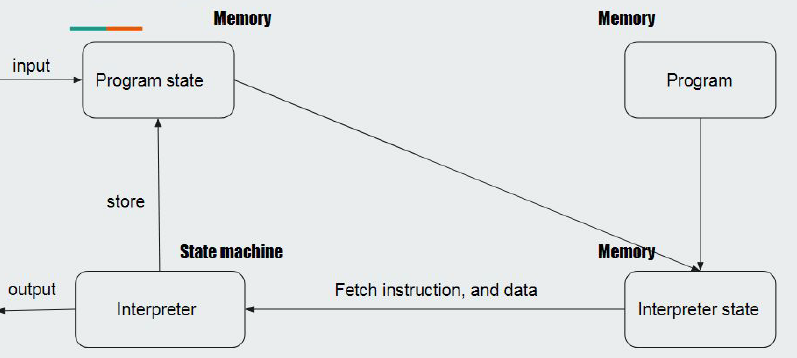
\includegraphics[width=0.4\textwidth]{./interpreter}
\end{center}
